% Numerical Computing II
% Homework 18

\documentclass[11pt]{article}
\usepackage{listings}
\usepackage{amsmath}
\usepackage[inside]{coordsys}
\usepackage{amsfonts}
\usepackage{graphicx}
\begin{document}         
% Start your text
\newcommand{\makehomework}[2]%
{\begin{center}%
	\Huge #1\\%
	\Large #2\\%
	Marty Fuhry\\%
	\today%
\end{center}}
\makehomework{Numerical Computing II}{Homework 18: Quadrature}

\lstset{language=Matlab,numbers=left,frame=single,breaklines=true,morecomment=[l]{//}}

\section*{Exercise 18.2}
We're looking to determine weights $w_1, w_2, w_3$ such that
\begin{align*}
    \int_0^1 f(x), dx \approx f(x_1)w_1 + f(x_2)w_2 + f(x_3)w_3
\end{align*}
integrates quadratic polynomials exactly. That is, we want to determine weights that solve a system of equation where each weight contributes to perfectly integrate up to a quadratic polynomial. So we need to solve the system:
\begin{flalign*}
    w_1 + w_2 + w_2 &= b - a\\
    x_1 w_1 + x_2 w_2 + x_3 w_3 &= \frac{1}{2}(b^2-a^2)\\
    x_1^2 w_1 + x_2^2 w_2 + x_3^2 w_3 &= \frac{1}{3}(b^3 - a^3).
\end{flalign*}
We are given $x_1 = 0, x_2 = \frac{1}{2}, x_3 = 1$ and $a = 0, b = 1$. Then, we can use 
\begin{align*}
    \begin{bmatrix}
        1 & 1 & 1\\
        0 & 1/2 & 1 \\
        0 & 1/4 & 1
    \end{bmatrix}
    \begin{bmatrix}
        w_1\\
        w_2\\
        w_3
    \end{bmatrix}
    =
    \begin{bmatrix}
        1\\
        1/2\\
        1/3
    \end{bmatrix}
\end{align*}
which corresponds to the Octave code:
\pagebreak
\lstinputlisting{problem_18_2.m}
This will yield the solution vector
\begin{align*}
    \begin{bmatrix}
        w_1 \\
        w_2 \\
        w_3 \\
    \end{bmatrix}
    =
    \begin{bmatrix}
        1/6\\
        2/3\\
        1/6
    \end{bmatrix}.
\end{align*}
This means, we can say with exactness, if $f(x)$ is a quadratic polynomial or less, then
\begin{flalign*}
    \int_0^1 f(x)dx &= f(x_1)w_1 + f(x_2)w_2 + f(x_3)w_3\\
                      &= \frac{1}{6}f(0) + \frac{2}{3}f(\frac{1}{2}) + \frac{1}{6}f(1)
\end{flalign*}

This will not integrate polynomials of higher degree exactly. This is because in the linear system of equations we solved, that is, the Vandermonde matrix with exactly three rows and three columns, we did not have enough data to force our weights to line up exactly with higher degree polynomials. If we had more data points, $x_i$, we would be able to determine weights which could integrate higher degree polynomials exactly. If we wanted to interpolate a third degree polynomial exactly, we would need a fourth weight.
If we had a fourth weight, $w_4$, we would need a fourth node $x_4$ to solve for the fourth weight, and thus, we would need the function evaluated at that fourth node.

\pagebreak
For the interval [1,2], we perform a change of variables. We define the function $x(t)$ on the interval [-h,h] where $h \in \mathbb{R}$. We say $x(-h) = 1$ and $x(h) = 2$. Then, the function $x'(t) = \frac{1}{2h}$. We also define the function $g(t)$ such that:
\begin{flalign*}
    g(t) &= f(x(t))\implies \\
    \int_1^2 f(x)dx &= \int_{-h}^{h} f(x(t))x'(t)dt\\
                     &= \int_{-h}^{h} g(t)\frac{1}{2h}dt\\
                     &= \frac{1}{2h} \int_{-h}^{h} g(t)dt\\
                     &\approx \frac{1}{2h} (w_1 g(-h) + w_2 g(0) + w_3 g(h))\\
                     &\approx \frac{1}{2h} (w_1 f(1) + w_2 f(1/2) + w_3 f(2))
\end{flalign*}
Now, remembering from our system of equations for solving $f(t) = t$ and $f(t) = t^2$,
\begin{flalign*}
    -w_1 h + w_3 h &= 0\\
    w_1 + w_3 &= \frac{2h}{3}
\end{flalign*}
We solve for $w_1 = w_3 = \frac{h}{3}$ and from $w_1 + w_2 + w_3 = 2h$, we solve $w_2 = \frac{4h}{3}$. Then,
\begin{flalign*}
    \int_1^2 f(x),dx &\approx \frac{1}{2h} (w_1 f(1) + w_2 f(1/2) + w_3 f(2))\\
                     &\approx \frac{1}{2h} (\frac{h}{3} f(1) + \frac{4h}{3} f(1/2) + \frac{h}{3}f(2))\\
                     &\approx \frac{1}{6} (f(1) + 4f(1/2) + f(2))
\end{flalign*}


\pagebreak
\section*{Exercise 18.4}

The interval [-10,10] may be evaluated at 4 points like this using $N = 4$:

\begin{center}
\setlength{\unitlength}{.2in}
\begin{picture}(10,2)(-3,-1)
    \numbline[1]{-10}{11}
    \interval[-7.5,-7.5]
    \interval[-2.5,-2.5]
    \interval[2.5,-2.5]
    \interval[7.5,7.5]
\end{picture} 
\end{center}
Now, a naive approach to reevaluating the function for $N = 8$ points would try something like this:
\begin{center}
\setlength{\unitlength}{.2in}
\begin{picture}(10,2)(-3,-1)
    \numbline[1]{-10}{11}
    \interval[-8.75,-8.75]
    \interval[-6.25,-6.25]
    \interval[-3.75,-3.75]
    \interval[-1.25,-1.25]
    \interval[1.25,1.25]
    \interval[3.75,3.75]
    \interval[6.25,6.25]
    \interval[8.75,8.75]
\end{picture} 
\end{center}
But none of the points have matched up from the second evaluation! We have to reevaluate every single point! This is terrible, and clearly not a good way to proceed.

Luckily, we can easily rectify this by simply "shifting" the points from the second evaulation to line up with the first evaulation, like this:
\begin{center}
\setlength{\unitlength}{.2in}
\begin{picture}(10,2)(-3,-1)
    \numbline[1]{-10}{11}
    \interval[-7.5,-7.5]
    \interval[-2.5,-2.5]
    \interval[2.5,-2.5]
    \interval[7.5,7.5]
    \interval[-5.0,-5.0]
    \interval[0,0]
    \interval[5,5]
    \interval[10,10]
\end{picture} 
\end{center}
Now we only need to evaulate 4 more points: $f(-5),f(0),f(5),f(10)$ and reusing the old points we evaluated for the previous quadrature evaluation. In general, to double $N$, we need only compute $N$ more points.

This method of reusing old points works very well when we need to go "backwards", too. That is, say we have already computed $N$ points for some evaluation. Now we want a worse precision (for some reason or other) by only counting $N/2$ points. Why would we ever want to do this, you ask? I have no idea. Still, we can simply reuse the old points by "shifting" our evaluation to make them line up, and never have to compute more points if we go "backwards" in our accuracy. 

\section*{Exercise 18.5}



\section*{Exercise 18.6}

\section*{Exercise 18.7}

% Import Program 
%\lstinputlisting{problem_17_1.m}

% Import Graph
%\begin{center}
%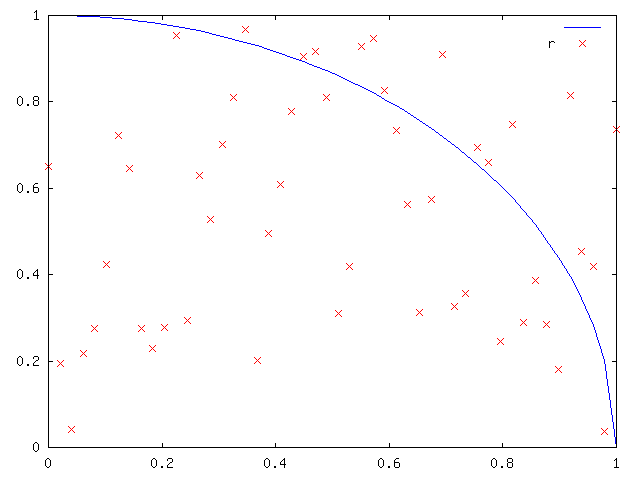
\includegraphics[scale=0.5]{problem_17_1_graph.png}
%\end{center}

% Stop your text
\end{document}
